
\documentclass[paper=a4,font size=10pt]{scrartcl}

\usepackage{titlesec}
\usepackage[english]{babel}															% English language/hyphenation
\usepackage[protrusion=true,expansion=true]{microtype}	
\usepackage{amsmath,amsfonts,amsthm} % Math packages
\usepackage{graphicx}	
\usepackage{url}
\usepackage{float}

%%% Custom sectioning
\usepackage{sectsty}
\titleformat{\section}
{\normalfont\Large\bfseries}{\thesection}{1em}{}
\titleformat{\subsection}
{\normalfont\large\bfseries}{\thesubsection}{1em}{}
\titleformat{\subsubsection}
{\normalfont\normalsize\bfseries}{\thesubsubsection}{1em}{}
\titleformat{\paragraph}
{\normalfont\normalsize\bfseries}{\theparagraph}{1em}{}




%%% Custom headers/footers (fancyhdr package)
\usepackage{fancyhdr}
\pagestyle{fancyplain}
\fancyhead{}											% No page header
\fancyfoot[L]{}											% Empty 
\fancyfoot[C]{}											% Empty
\fancyfoot[R]{\thepage}									% Pagenumbering
\renewcommand{\headrulewidth}{0pt}			% Remove header underlines
\renewcommand{\footrulewidth}{0pt}				% Remove footer underlines
\setlength{\headheight}{5pt}
\setcounter{secnumdepth}{5}
\usepackage[headheight=5pt,headsep=0pt,textheight=690pt]{geometry}


%%% Equation and float numbering
\numberwithin{equation}{section}		% Equationnumbering: section.eq#
\numberwithin{figure}{section}			% Figurenumbering: section.fig#
\numberwithin{table}{section}				% Tablenumbering: section.tab#



%%% Maketitle metadata
\newcommand{\horrule}[1]{\rule{\linewidth}{#1}} 	% Horizontal rule

\title{
		%\vspace{-1in} 	
		\usefont{OT1}{bch}{b}{n}
		\normalfont \normalsize \textsc{B565 Data Mining} \\ [10pt]
        \normalfont \normalsize \textsc{School of Informatics and Computing} \\ [10pt]
         \normalfont \normalsize \textsc{Indiana University} \\ [20pt]
		\horrule{0.5pt} \\[0.4cm]
		\huge Kaggle Microsoft Malware Classfication Challenge \\
		\horrule{2pt} \\[0.5cm]
}
\author      
{Puneet Loya, Suhas Gulur Ramakrishna, Vidhixa Joshi\\
        \normalsize
        \today
}
\date{}
	 
%%% Begin document
\begin{document}
\maketitle

\newpage

\tableofcontents

\newpage 

\section{Abstract}
In recent years the malware industry has become a well-organized market for involving large amounts of money funded towards protection and mitigation of malware attack on machines ranging from personal computers to large scale systems. Every year millions of dollars are lost due to malware attack that the systems could not necessarily see as a threat. This challenge brought to attention the need to effectively analyze and classify malware files so as to create a future for smarter anti-virus solution and thereby protection systems with the efforts by data science community.


\section{About the Company} 

Fantastic 3 is a company of three enthusiastic data miners determined to make a break through by their skills and endurance. The motto of the company is to help the computer users to be able to carry out all tasks without being skeptical about malwares existing in the System. The organization members are:
\begin{enumerate}
	\item Puneet Loya: A skilled software polyglot, can work on almost any platform existing. He has gained expertise in text mining.
	\item Suhas Gulur Ramakrishna: A specialist in R, an algorithmic expert and great understanding of IDA and Malware. He is a domain expert.
	\item Vidhixa Joshi: A great planner with good multi-tasking skills. Experienced python developer, a quite helpful skill required in data science. 
\end{enumerate}


\section{Project Contract}

We are extremely thankful to \textbf{ ACME Dynamic General Systems } for giving us an opportunity to deal with the Malware that effect their systems. The software has been installed in Multiple Systems at Zoo. Over a period, there have been multiple attacks on the Systems with a variety of Malwares. There are 20 different computer programs running at the Zoo, with each producing its own logs.
These logs have been examined and scenarios have been reproduced to obtain detailed information regarding the malwares. A brief overview of these Malwares is discussed in the following section.

\section{Executive Summary}

\subsection{Project Outline}

A malware \cite{microsoft} or a software intended to damage or disable computer or computer systems is still a big challenge faced by the tech industry. Most commonly used tools that is used to prevent a malware are anti-virus and anti-spyware software. An anti-virus is an essential part of multi-layered security strategy. There is a constant stream of vulnerabilities from browsers, plug-ins and operating system itself. 
\newline
\newline
The way these anti-virus work \cite{antiVirus} is by scanning the files in background, real-time many a times, to compare the behavior against its known virus, worm, spyware type. It also does “heuristic” checking in which bad behavior is monitored and if there is threat to system, the user is alerted. Thus it is essential to recognize the various forms of virus to be able to protect against their attack.It is equally important to understand the pattern of each known virus type and categorize them to be able to detect a polymorphic form of virus encountered in future. This is the basic motivation that the problem could be solved by data mining.
\newline
\newline
The malwares \cite{surveyMalware} are broadly classified into 9 families namely Ramnit, Lopllipop, Kelihosver3, Vundo, Simda, Tracur, Kelihosver1, Obfuscator.ACY and Gatak. Raw data contained 10,868 files of different malware samples worth 17.252GB gziped data. Raw data contains hexadecimal representation of file’s binary and corresponding metadata log consisting of function calls, strings, generated by IDA tool.


\subsection{Past Work and Shortcomings}

Anomaly-based detection and specification-based detection are more real time malware identifying techniques. Specification-based detection is a sub-type of anomaly-based detection. In anomaly-based detection technique, the system is being monitoring continuously and any anomalous behavior by a running program is brought to attention and fixed. The knowledge of differentiating anomalous vs normal behavior comes from a set of rules or check-list that is maintained by the detecting software. Advantage of this technique is that it dynamically can detect suspicious program behavior and classify it was malware. Disadvantage is that it does not learn from what it experiences. It cannot handle malware that cause sudden attack without gradually displaying anomalous behavior. In specification-based detection, again would abide by a set of rules which checks valid behavior of program. Violation of which is considered a threat and potential malware. Again, the disadvantage is that there is no learning involved. 
\newline
\newline
Signature-based \cite{surveyMalware} detection uses characterization of what is known as malicious to detect existence of malware in system. These signatures are learnt over the years by analyzing every new sample of malware detected. Matching against these signatures or even a higher percentage of it is an indication of malware presence. Machine learning plays a heavy role in this type of detection. Classification/categorization is identifying differences between objects or data in a dataset and training over them. Disadvantage is that there will always be false positives and false negatives.

\subsection{Data Description}
Grouping different malware into their respective classes is a challenging task. If unsupervised learning method was used to find the class with which the data belongs then we would end up so many families of malwares. On closer look on these families they can be related to each other and can be classified under one parent family.  Note that this unsupervised training will generally fit into the decision problem framework because the goal is not to produce a classification but to make decisions that maximize rewards. However, with huge number of installation and massive amount of attacks happening every minute it is advisable to tackle these virus as a class of family than treating it as one separate individual virus. Thus classification of malware into predefined classes (supervised) is preferred over unsupervised learning. Microsoft receives millions of virus everyday making it very difficult classify each of them. Moreover each malware is a polymorphic version of other viruses of same family to avoid detection of them. Hence, Microsoft has provided the data science community with trained dataset and test dataset of malwares. 
\newline
\newline
Both training set and test set consists of nearly 11000 malwares. Each malware is identified by unique 20 character code. There are two files for each malware - asm and bytes file. The asm file is the meta information obtained from dump and binary files extracted from standard IDA assembler tool. These files contain microprocessor(x86) execution of instructions, subroutine, memory allocation, variable manipulation, etc. The bytes file is the raw hexadecimal representation of the malware’s binary content.   
\newline
\newline
As part of pre-Analysis the count of each files in a family for train dataset was observed. The distribution is given in image below. We found that class 1, 2 and 3 were significantly more compared to others. Class 5 files were less than 50 making it insignificant in the classification. This kind of gave intuition of how diverse the files are which helped in predicting the test data as well. 
\newline
\begin{figure}
	\begin{center}
		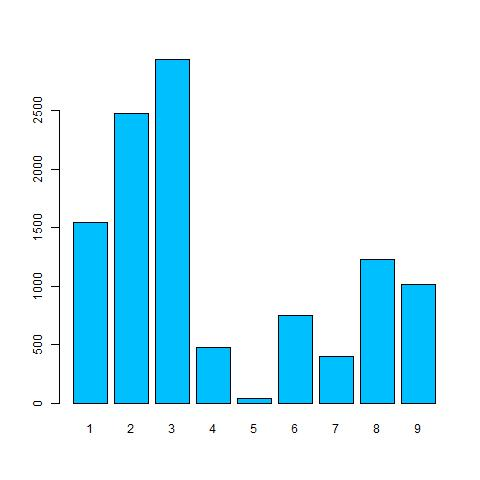
\includegraphics[height=7cm,width=7cm]{figures/classFrequencies.jpg}
	\end{center}
\end{figure}

The size of files also varied from couple of MB’s to 80 MB. The over-all size of the complete data including train files and text files amounted to nearly 500 GB. 

\subsection {Strategy}
Considering the huge training data, it was important to concise the data to relatively smaller size from which features can be extracted.   We tried to detect the signature in form of patterns in set of instructions and sequence of bytes. We further worked on making our feature vector better by reducing the dimension of feature vector and train our classification model. Dataset being this large, it provided us a huge ballpark to play in. 
\subsubsection{Instruction  and Byte Proportion Based detection}
\paragraph {Data Transformation} \mbox{} \\

We tried to look deep into asm files to pick patterns which matter in feature selection.  The rest can be neglected, thereby reducing the computation time of extracting features. Initially we took few very prominent instructions like (mov, push, etc.) and tried plotting the frequency graph of these instruction with few malwares ranging across all classes. On observation, the proportion of instruction say mov to push was nearly constant for a particular class.  In the images below are two examples of classes have unique slope for mov to push instruction. This intuition led us to calculate the ratio of each instruction in the file to sum of all instruction in that file. This is almost constant for a particular class of files. When plotted, each instruction in a class has slope nearly equal to zero.  This means for all the files in particular class, proportion of each instruction to total count of instruction is constant. 

\begin{figure}[H]
	\begin{flushleft}
	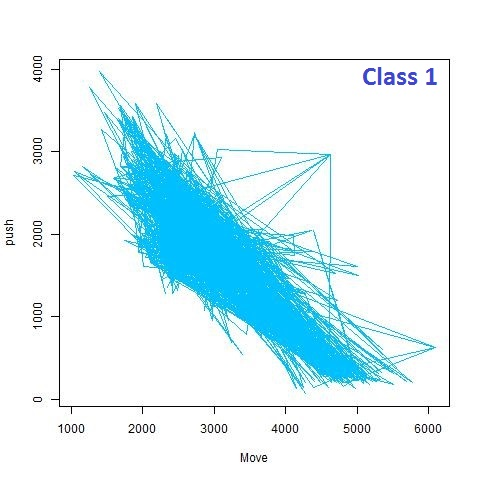
\includegraphics[height=7cm,width=7cm]{figures/class1MovPush.jpg}
	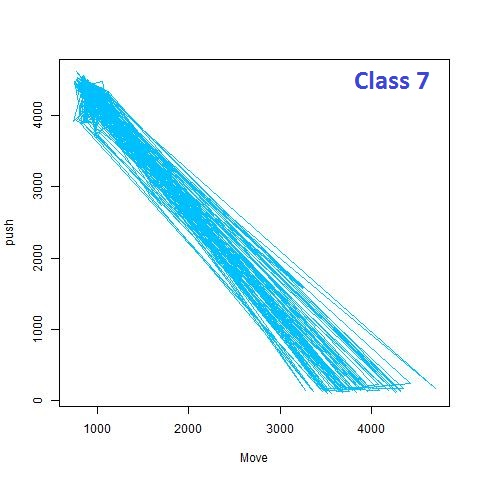
\includegraphics[height=7cm,width=7cm]{figures/class7MovPush.jpg}
	\end{flushleft}
\end{figure}

So we decided upon consolidating the 500 GB data into files of proportion of each instruction to sum of all instruction in that file.  x86 architecture had approximately 150 instructions. While running the code for entire test and train data we found that few files doesn’t have any instruction within them. To overcome that case we took the help of Bytes file which will be discussed further.
\newline
\newline
The total consolidation of test and train data came down to 20 MB. Similarly, bytes file also contain byte address codes ranging from 00 to FF (total of 257 including “??”) . The proportion of each Byte code to count of all Byte codes is taken. This transformation of data for both and test data came up to 80 MB. 

\paragraph {Feature Selection} \mbox{} \\

For the train data right now we had around 11000 files. Each file consisted of:
\begin{enumerate}
\item 150 instruction features:  Of 150 features most instruction didn’t have presence in almost all the files. So keeping a threshold of 1\% in each file, instructions which fall less than that was eliminated. This brought down features from 150 down to 47. Further, correlation between these 47 features was computed and in each pair having correlation more than 0.7 one was eliminated based on whose information gain was less. The instructions came down from 47 to 33. 
\item 257 byte- count: As similar to above case a threshold of 1\% is kept for Byte proportion as well. Correlation check between two features were done and in each pair having correlation more than 0.7 one was eliminated based on whose information gain was less. The features came down from 257 to 244. On combining the total features came up to (33 + 244) = 277. 
\end{enumerate}

\paragraph{Classfier} \mbox{} \\

We used Random Forest classifier for the input. Random forest classifier suits well for the huge data and the output format was to be given in the probabilities of a file belonging to each class. This requirement is well handled by Random Forests itself as it internally does voting of each file.  Random Forest in R is used for training. To create probabilities of output and also reduce the time in building one big Random Forest (of 500 trees and 50 random features).  To reduce the burden on one Random forest, a cross validated Random Forest is trained. This function was written completely in R specific to our project. 
Cross Validated Random forests consisted of 20 random forests. Each random forest is trained on 30\% of entire data with replacement (Bootstrap approach). The test data is it is fed into 20 trained Random Forests. Each random forest will predict a class. The probability of that particular test file for that class is calculated based on number of trees each predicting that class to total number of trees.   

\paragraph{Prediction} \mbox{} \\
For each testing file, those features removed from asm and bytes files of training is removed and then tested on the Random Forests trained.

 
\subsubsection{N-gram based appraoch}
On manual inspection of a few asm files of a class, the subroutines called within a file appeared to have a similar set of instructions in the same order. So an intuition was, similar ordered instructions may try to cause similar attack being in a family. Hence frequency of similar ordered instructions could be a distinguishable feature of a class. For this, all unique 4-grams i.e, 4 opcodes appearing in order were considered. We did not consider 2-gram or 3-gram because of three reasons: 
\begin{enumerate}
\item[$\bullet$]2-gram or 3-grams would produce huge features which would be difficult to evaluate and trusting.
\item[$\bullet$]2-gram  or 3-grams may produce less substantial evidence as 4-grams.  
\item[$\bullet$]According to the research \cite{santos2009n}, 4-gram has been quite optimal detection of signature.
\end{enumerate}

\paragraph{Data Cleaning and Pre-processing} 
\begin{enumerate}
	
\item[$\bullet$]Each line in the asm file is parsed to extract opcode using regular expression.
\item[$\bullet$]The dictionary of known opcodes is maintained a prior. 
\item[$\bullet$]After a file is parsed, it is written to a lucene index \cite{luceneLibrary}.
\item[$\bullet$]The lucene index stores opcodes in an n-gram (4-gram) format. Lucene is preferred because it reduces effort during data transformation.
\item[$\bullet$]The parsing is done in a multi-thread manner with each thread responsible for a file.
\item[$\bullet$]Using MySQL all the files belonging to a class are retrived and indexed. 
\item[$\bullet$]The above process is run for each class separately for trained data.
\item[$\bullet$]For the test data, similar procedure is followed except that files are picked as a set 1000 files (No class label yet).
\end{enumerate}

\paragraph{Feature Selection and Data Transformation}
\begin{enumerate}
\item[$\bullet$]For the trained data, the count of unique 4-grams for each class label is calculated.
\item[$\bullet$]A maximum for n-gram frequencies for all classes is obtained using the lucene index.
\item[$\bullet$]On plotting the histogram, the n-gram with frequencies more than 70000 were quite few and hence discarded. The plot between Minimum frequencies to the coressponing unique number of n-grams for each class is constructed. The lower limit was assigned per class by observing this plot.

\begin{figure}
	\begin{flushleft}
	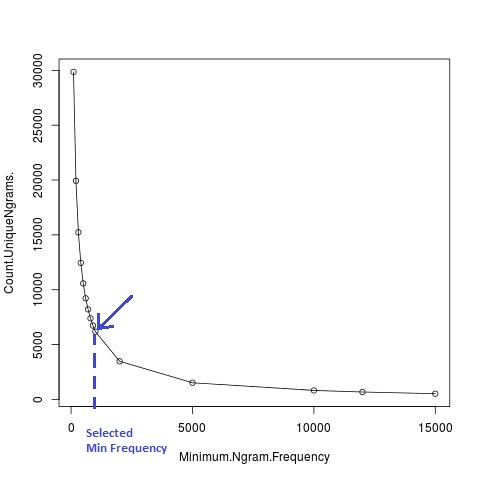
\includegraphics[height=7cm,width=7cm]{figures/class1.jpg}
	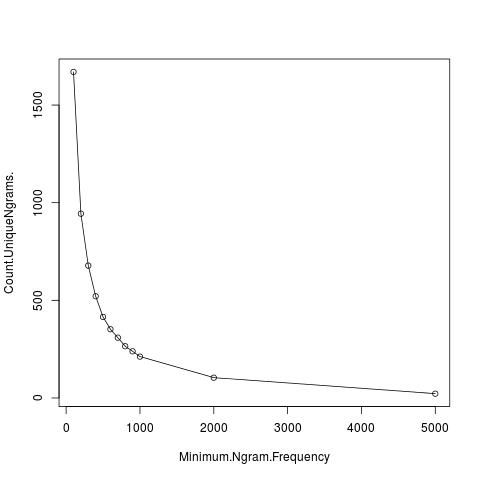
\includegraphics[height=7cm,width=7cm]{figures/class7.jpg}	
	\end{flushleft}
	
\end{figure}

\item[$\bullet$]As expected, the plot shows inverse behavior of minimum frequency to the count of unique n-grams. In this plot, we choose a point where there is a sharp decrease in number of n-grams. The corresponding minimum frequency count is chosen as lower limit for that class. This is repeated for all the 9 classes.  
\item[$\bullet$]The union of all n-grams obtained from these 9 classes is taken as the feature set. The size of this feature set was 6250. Keeping a correlation threshold of 0.5 and information gain of greater than zero, the feature set was reduced from 6250 to 1017. Therefore the opcode feature set contained 1017 4-grams. 
\item[$\bullet$]But these features are not enough because there are files with no opcodes and the classifier will make a wild guess as there is no opcode n-grams for these files. Hence, byte proportion features which is used in first approach was reused. 
\item[$\bullet$]Out of the 257 features of byte proportions, few features were eliminated using correlation. Hence this byte feature set was reduced to 244. The training feature sets of opcode n-gram and byte frequency are merged based on the filename resulting in total of 1261 features. 
\item[$\bullet$]From the test data, the information for the opcode feature set was extracted using lucene index. The byte frequency test data calculated during the previous approach is also used. The feature sets for test are then merged as above. 
\end{enumerate}

\paragraph{Training and Testing} \mbox{} \\
For training, the Random Forest Classifier is used. It is built using the python scikit-learn \cite{scikit-learn} package. The random forest classifier was trained on the training data starting with 150 trees. The number of features considered for node split by default is square root of total features picked randomly with bootstrap sampling. This classifier was then tested with the test set. Later with experimentation of the random forest training API the model was optimized by using 500 trees and 500 features for node split to get a log loss of \textbf{0.064}.

\paragraph{Feature Vector Reduction Efforts} \mbox{} \\
To reduce the size of feature set we use three tehcnique. Use manual inspection of features, Correlation matrix and PCA. 

\begin{enumerate}
\item[$\bullet$]Correlation threshold set to 0.7 based on various trials. This reduced the feature vector but with  correlation we get cannot be certain about which feature to discard given the are highly correlated to ech other.
\item[$\bullet$]PCA helps solve this problem. We use the R package with function prcomp that performs PCA over given dataset and presents results in a plot showing contribution of each PC in defining whole set. By visually inspecting the plots for asm and bytes file, we concluded that top 79 of asm PCs and 69 of bytes PCSs help contribute to about 98 percent of train set examples.
\item[$\bullet$]Log loss higher that correlation. 0.07 on cross validation.
\end{enumerate}

\subsubsection{Outcome}
\begin{enumerate}
	
\item[$\bullet$] The following table summarises the accuracy of our approaches.

\begin{tabular}{ | l | l | l | }
	\hline
	Approach & Number Of Features & Log Loss \\ \hline
	Instruction  and Byte Proportion based detection & 277 & \textbf{0.13} \\ \hline
	N-gram based detection & 1017 & \textbf{0.11} \\ \hline
	N-gram with Byte Proportion based detection & 1261 & \textbf{0.064} \\ \hline
\end{tabular}
\item[$\bullet$] Both asm and bytes files together are important for creating feature vector.
\item[$\bullet$] Cross validation of train files help remove bias while creating trees in random forest.
\item[$\bullet$] Correlation gave better results that PCA. The reason could be that PCA is not a statistical method from the viewpoint that there is no probability distribution specified for the observations made. Therefore it is important to keep in mind that PCA
best serves to represent data in simpler, not to chop off dimensions.
\end{enumerate}

\section{Future}
\begin{enumerate}
\item[$\bullet$] The other supervised learning techniques like Naïve Bayes, Logistic regression and  Support vector machine can be used to see which technique fits best. We went ahead with Random forest as it is well suited for huge data. But there might be neat advantages in above mentioned approaches that can produce better results.
\item[$\bullet$] The features selected for first approach was very less. There is always more scope for find more features and better features.
\item[$\bullet$] As observed, few asm files lacked instructions, meaningful information can be obtained by finding the relation between bytes and asm files. So far we have used it as two separate files than treating it as a relative functions. If we are able to map these two files, features extraction will be easier and results may be better.   
\item[$\bullet$] Better techniques for feature selection like ridge regression can be used. Using correlation along with information gain to remove features may not produce the feature subset.
\end{enumerate}


\section{Appendix}
\subsection{Logloss}
This is the multi-class version of the Logarithmic Loss metric \cite{kaggleCite}. Each observation is in one class and for each observation, you submit a predicted probability for each class. The metric is negative the log likelihood of the model that says each test observation is chosen independently from a distribution that places the submitted probability mass on the corresponding class, for each observation.

\subsection{Approach tried with equal weightage to all classes}
As per the predictions from the first approach, the files of a class whose count was very less (example class 5) was failing drastically as bootstrap which picks 30\% of entire data for the first approach will pick few files. To overcome, an attempt was made by giving equal number of files of each class while training Random Forest. This helped in improving accuracy of those classes which initially had lesser files but the accuracy of classes which have a higher number started to reduce. Since the testing data also have more files of classes which had more count in training, the log loss increased to 0.16 compared to 0.13 in the first aprroach. We realized this was an incorrect approach and didn’t proceed in this direction.   	

\subsection{Lucene}

Apache Lucene is a sub-flagship project for data indexing using Java. It is a higly developed library with various text mining algorithms.

\subsection{Code}

All the code written is attached as an archive with the project.

\bibliographystyle{plain}
\bibliography{references}

\end{document}